%% Beginning of file 'sample631.tex'
%%
%% Modified 2021 March
%%
%% This is a sample manuscript marked up using the
%% AASTeX v6.31 LaTeX 2e macros.
%%
%% AASTeX is now based on Alexey Vikhlinin's emulateapj.cls 
%% (Copyright 2000-2015).  See the classfile for details.

%% AASTeX requires revtex4-1.cls and other external packages such as
%% latexsym, graphicx, amssymb, longtable, and epsf.  Note that as of 
%% Oct 2020, APS now uses revtex4.2e for its journals but remember that 
%% AASTeX v6+ still uses v4.1. All of these external packages should 
%% already be present in the modern TeX distributions but not always.
%% For example, revtex4.1 seems to be missing in the linux version of
%% TexLive 2020. One should be able to get all packages from www.ctan.org.
%% In particular, revtex v4.1 can be found at 
%% https://www.ctan.org/pkg/revtex4-1.

%% The first piece of markup in an AASTeX v6.x document is the \documentclass
%% command. LaTeX will ignore any data that comes before this command. The 
%% documentclass can take an optional argument to modify the output style.
%% The command below calls the preprint style which will produce a tightly 
%% typeset, one-column, single-spaced document.  It is the default and thus
%% does not need to be explicitly stated.
%%
%% using aastex version 6.3
\documentclass[linenumbers, twocolumn]{aastex631}

\newcommand{\vdag}{(v)^\dagger}
\newcommand\aastex{AAS\TeX}
\newcommand\latex{La\TeX}

\newcommand{\Msun}{\ensuremath{M_{\odot}}}
\newcommand{\yr}{\ensuremath{\textrm{yr}}}
\newcommand{\kpc}{\ensuremath{\textrm{kpc}}}
\newcommand{\pc}{\ensuremath{\textrm{pc}}}

%% Reintroduced the \received and \accepted commands from AASTeX v5.2
% \received{March 1, 2021}
% \revised{April 1, 2021}
%\accepted{\today}

\shorttitle{The CGM of Merging Galaxies}
\shortauthors{Beane et al.}

\graphicspath{{./}{fig/}}

\begin{document}

\title{Stimulated Accretion from Circumgalactic Media Interactions}

\author{Angus Beane}
\affiliation{Center for Astrophysics $|$ Harvard \& Smithsonian,  Cambridge, MA, USA}

\author{Federico Marinacci}
\affiliation{Department of Physics \& Astronomy `Augusto Righi', 
University of Bologna, Bologna, Italy}

\author{Lars Hernquist}
\affiliation{Center for Astrophysics $|$ Harvard \& Smithsonian,  Cambridge, MA, USA}

\author{others}

%% Mark off the abstract in the ``abstract'' environment. 
\begin{abstract}
  It is now well-established that galaxies host extended gaseous haloes dubbed
  the circumgalactic medium (CGM) which play a critical role in receiving and
  providing gas from and to the disk. Typically metal-poor, the CGM is a major
  actor in the nuclear abundance evolution of galaxies. While aspects of
  isolated CGM, such as its rotation and multiphase nature, have been studied,
  the interaction between the CGM of two merging galaxies is less well
  understood. In this work, we present hydrodynamic simulations of a controlled
  galaxy merger, roughly resembling a merger the Milky Way experienced early in
  its history. Unsurprisingly, the CGM of the satellite galaxy is stripped early
  in the merger -- mostly during its first pericentric passage (check). This has
  the effect of stimulating the accretion of gas from the host's CGM onto its
  disk. This occurs due to two effects: (1) Cold gas from the satellite's CGM
  mixes with gas in the host's CGM and cools it to a regime where cooling is
  more efficient, thus reducing the gas' thermal pressure support. (2) The
  satellite deepens the potential well of the host galaxy, reducing its
  free-fall time. These effects combine to enhance the accretion of gas onto the
  host's disk. In our setup (for which there is significant uncertainty), the
  bulk amount of gas accreted on the disk can increase by a factor of $\sim2$
  (\textcolor{red}{checl}).
\end{abstract}

%% Keywords should appear after the \end{abstract} command. 
%% The AAS Journals now uses Unified Astronomy Thesaurus concepts:
%% https://astrothesaurus.org
%% You will be asked to selected these concepts during the submission process
%% but this old "keyword" functionality is maintained in case authors want
%% to include these concepts in their preprints.
\keywords{Classical Novae (251) --- Ultraviolet astronomy(1736) --- History of 
astronomy(1868) --- Interdisciplinary astronomy(804)}

\section{Introduction} \label{sec:intro}
The present day Milky Way formed through a combination of external interactions
and internal secular evolution. Disentangling the role and importance of each is
a major goal of Galactic science today.

The last\footnote{i.e., not ongoing} significant merger was between the
proto-Milky Way disk and the {\em Gaia}-Sausage-Enceladus (GSE)
(\textcolor{red}{spell check}) satellite galaxy. The stellar debris from this
merger constitutes $\sim50\%$ \textcolor{red}{check} of the inner ($r<?\,\kpc$)
stellar halo. It may have also led to a tilted, triaxial dark matter halo
(\textcolor{red}{cite}).

The GSE merger is often invoked (\textcolor{red}{cite}) to explain the observed
bimodality in the \textcolor{red}{alpha iron} abundance plane
(\textcolor{red}{cite}). Because GSE-mass galaxies are expected to have a lower
star formation efficiency than proto-Milky Way-mass galaxies
(\textcolor{red}{cite}), the gas from GSE should be relatively metal poor. The
gas from GSE thus dilutes the gas in the proto-Milky Way, ``resetting'' the
chemical abundance of the Milky Way.

However, it has also been claimed that the \textcolor{red}{alpha iron}
bimodality can be explained through secular processes. \textcolor{red}{Sentence
explaining the basic concept.} The argument is not that the GSE merger did not
happen, but rather that it is not {\it necessary} and might not even be {\it
sufficient} to explain the bimodality. Ongoing work to detect the bimodality in
external galaxies may shed further light on the topic (\textcolor{red}{cite}).

Investigating GSE-like mergers in cosmological simulations is a rich and active
area of research. Many mergers believed to be similar to the GSE merger have
been identified in the literature (\textcolor{red}{cite}). \textcolor{red}{Blah
blah argue blah blah. And also blah blah argues blah blah.}

While much has been learned from GSE-like mergers in cosmological simulations,
they are not conducive to controlled experiments. It is possible to change the
mass of satellites through genetic modification (\textcolor{red}{Pontzen}), and
the GSE analog can be removed entirely (\textcolor{red}{Cooke cite}). However,
to our knowledge, no method has been applied to change the orbital parameters of
such a merger. It is also somehwat unclear if the circumgalactic media of
proto-Milky Way mass galaxies at $z\sim2$ are properly simulated.

In this work, we present hydrodynamic simulations of a controlled merger between
a GSE analog and the $z\sim2$ proto-Milky Way. 

\section{Methods}\label{sec:methods}

\subsection{Gaseous Halos}\label{ssec:gashalo} 

The nature of the circumgalactic media of local galaxies remains largely
uncertain. It is unclear whether the constraints we have on the local universe
apply to the circumgalactic media of $z\sim2$ galaxies. Nonetheless, we persist.

We assume the CGM of the Milky Way and GSE can be modelled using a $\beta$ profile,
\begin{equation}
  \rho(r) = \rho_0 \left( 1 + \left(\frac{r}{r_c}\right)^2 \right)^{-\frac{3}{2}\beta}\textrm{.}
\end{equation}
However, a $\beta$-profile has been shown to be a reasonable fit to the density
profile of galaxy clusters and of the $L_{*}$ galaxy NGC 3221. Whether or not
such a profile extends to lower mass galaxies at $z~2$ is unclear, but to our
knowledge there is no better motivation for another profile.

Our construction of the Milky Way and GSE CGM follows
\citet{2023MNRAS.tmp.2070B}. In particular, we set $\beta=2/3$ and $r_c=0.22
r_s$, where $r_s$ is the scale length of the dark matter halo. For the Milky Way
and GSE, $r_c=9$, $6.5\,\textrm{kpc}$, respectively. For the present study we
keep $\beta$ and $r_c$ fixed and instead vary the central density $\rho_0$. Our
fiducial values are $9.61\times10^{-5}$ and $7.57\times10^{-5}\,\Msun/\pc^3$ for
the Milky Way and GSE, respectively.

A useful metric for assessing the central density is by the universal baryon
fraction $f_{\textrm{B}}$ -- i.e., the ratio between the mass in baryons to the
mass in dark matter within $R_{200}$ as compared to the mean ratio of the
universe.\footnote{To be explicit,
$f_{\textrm{B}}=(M_{\textrm{b}}/M_{\textrm{c}})/(\Omega_{\textrm{b}}/\Omega_{\textrm{c}})$,
where $M_{\textrm{b}}$ and $M_{\textrm{c}}$ are the mass of baryons and cold
dark matter within $R_{200}$, and $\Omega_{\textrm{b}}$ and
$\Omega_{\textrm{c}}$ are the mean baryon and cold dark matter densities of the
universe.} For our fiducial central densities, this value is $1.07$ and $0.28$
for the Milky Way and GSE respectively using the universal values from
\cite{2014AA...571A..16P}. An early argument by 


\begin{figure}
  \centering
  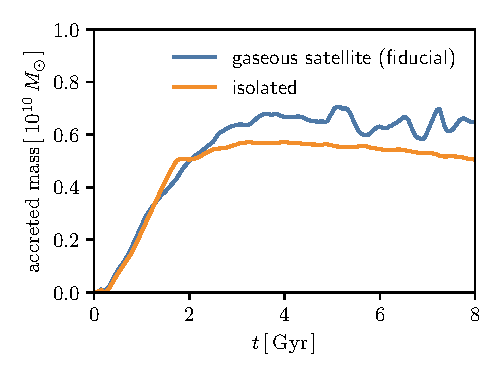
\includegraphics[width=\columnwidth]{fig/cumprof.pdf}
  \caption{The cumulative amount of the central's CGM gas accreted onto the disk
  ($r<20\,\kpc$) as a function of time. The blue line shows the case of the
  galaxy merger setup and the orange line shows the case of an isolated galaxy.
  The effect of the merger is to increase the amount of mass accreted onto the
  central. We stress that this plot does not include the mass from the satellite's
  disk or CGM.}
  \label{fig:cumprof}
\end{figure}

\bibliography{ref}{}
\bibliographystyle{aasjournal}

%% This command is needed to show the entire author+affiliation list when
%% the collaboration and author truncation commands are used.  It has to
%% go at the end of the manuscript.
%\allauthors

%% Include this line if you are using the \added, \replaced, \deleted
%% commands to see a summary list of all changes at the end of the article.
%\listofchanges

\appendix

\section{Modelling the Milky Way and GSE at $z=2$}


Our merger simulations are built upon reasonable models of both the Milky Way
and GSE at $z\sim2$. Much is uncertain about the properties of the Milky Way and
GSE at these redshifts.  We describe the motivation for the choices made in
constructing these models.

\subsection{The Milky Way}
We adopt a \citet{1990ApJ...356..359H} profile for our dark matter halo. For its
structural parameters, we follow \citet{2021ApJ...923...92N} and set its mass
and scale length to be $5\times10^{11}\,\Msun$ and $40.4\,\kpc$, respectively.
This matches a \citet{1996ApJ...462..563N} profile with
$R_{200}=129\,\textrm{kpc}$ and concentration $c_{200}=3.8$
(\textcolor{red}{check this}).

Milky Way-progenitor galaxies have been observed up to $z=?$ with well-formed
disks, and more massive galaxies have dynamically cold disks up to $z\sim6$. We
therefore assume the thick disk is settled and in place at $z=2$. We use the
structural parameters of the thick disk from . It is presently unclear if before
the GSE merger the Milky Way disk was already thickened, or if it was thickened
by the merger. Some simulations indicate that only prograde mergers efficiently
thicken disks (\textcolor{red}{check and cite}). For this work, we assume the
disk is already thick.

For the bulge, we assume the present day classical bulge was already in place at
$z=2$. Measurements of the structural parameters of the classical bulge are
uncertain due to contamination by the boxy peanut bulge generated by the bar
(\textcolor{red}{cite}). Some even argue that the classical bulge does not exist
(\textcolor{red}{cite}). Nonetheless, we assume the bulge properties from
\textcolor{red}{Bland Hawthorn, but check}. Specifically, we assume a Hernquist
bulge with $M_{\textrm{bulge}}=?$ and $a=?$.

We assume a gas disk with an exponential surface density profile and scale
length matched to the stellar disk. The vertical profile is set by the condition
of gravito-hydrostatic equilibrium as described in (\textcolor{red}{Springel}).
Varying the gas fraction of the disk strongly influences the SFR of the galaxy.
We therefore varied the gas fraction of the disk until we reached a target
SFR.\footnote{Note that when we varied the gas fraction of the disk, we kept the
mass (and scale length) of the stellar disk constant. Therefore, the total mass
of the disk changes as we vary the gas fraction.} \textcolor{red}{People} argue
that in order for the thick disk to have formed thick, the SFR of the disk at
$z\sim2$ needed to be $\sim15\,\Msun/\yr$. It is not necessary for the disk to
be thick at $z\sim2$, so we acknowledge this is an upper limit on the SFR. We
adopt an initial gas fraction of $0.7$ which results in an average SFR of
$\sim16\,\Msun/\yr$.

Finally, we note that the present day Milk Way has a well-formed bar. It is
expected to have formed within a few Gyr of the GSE merger, so it is unclear if
the bar formed before, as a result of, or after the merger. This is not a focus
of the current work. The presence of a classical bulge and the disk being
dynamically hot is sufficient for the disk to be stable against bar
instabilities.

\end{document}

% End of file `sample631.tex'.
